\subsection{Design of Symmetric-key Algorithms}

\renewcommand{\TITLE}{\it Design of Symmetric-key Algorithms}

\begin{frame}
\CurTitle{}

\vspace{1.25cm}

\Center{
    \large \textit{Lightweight} Cryptography:

    \vspace{0.25cm}

    \large Cryptography for \textcolor{red}{resource-constrained} devices \\
    (Internet of Things)
}
\end{frame}


\begin{frame}[t]
\CurTitle{}

\Center{
\hspace*{-1cm}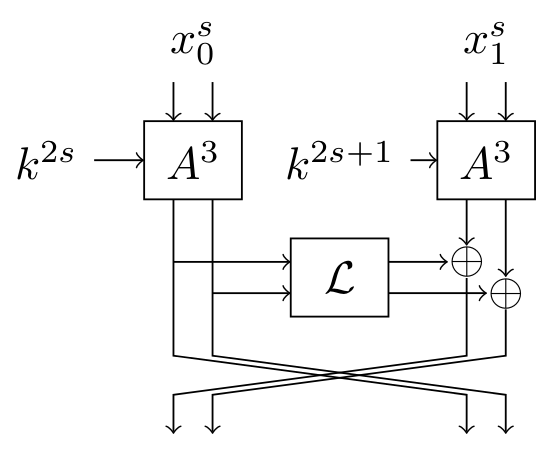
\includegraphics[height=5cm]{figures/Sparx-64-round-function.png}
}

\Center{
    \large \textbf{Sparx}: a \textit{lightweight} block cipher \\
    based on a \textcolor{red}{new design strategy}
}
\end{frame}


\begin{frame}[t]
\CurTitle{}

\Center{
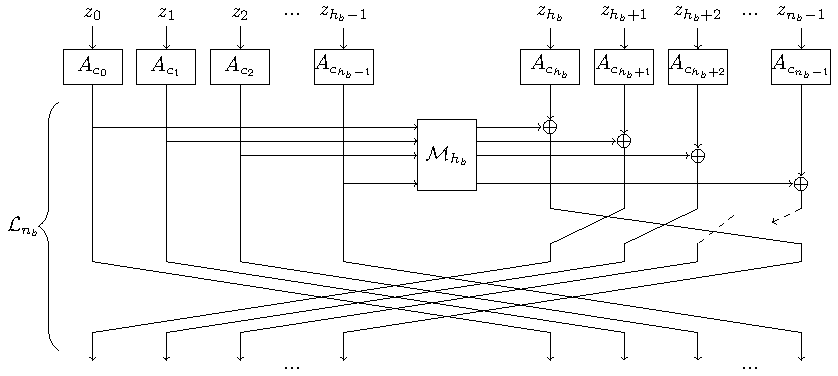
\includegraphics[height=5cm]{figures/step.pdf}
}

\Center{
    \large \textbf{Sparkle}, \textbf{Esch} and \textbf{Schwaemm}:
    
    cryptographic permutations, hash functions \\
    and authenticated encryption
}
\end{frame}


\begin{frame}
    % \begin{center}\Large Part IV. Publications\end{center}
    \begin{center}\Large \TITLE\end{center}
    
    \nocitepartiv{mybibSPARX}
    \nocitepartiv{mybibSPARKLE}
    \bibliographystylepartiv{unsrt}
    \bibliographypartiv{mybiblio.bib}
\end{frame}

\begin{frame}
\Center{\LARGE How to make sure \\
that an encryption scheme is \alert{secure}?
}

\Center{

\includegraphics[height=3cm]{lock.pdf}
% 
\includegraphics[height=3cm]{figures/locked.pdf}
% 
\includegraphics[height=3cm]{figures/unlocked.pdf}
}

\pause

\Center{
\LARGE \textcolor{blue}{Security Proofs} and \textcolor{red}{Cryptanalysis}!
}

\end{frame}

% ======================================================
\begin{frame}
\Title{\textcolor{blue}{Security Proofs: Modes and Structures}}

\Center{
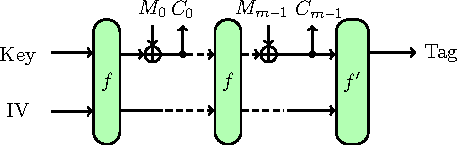
\includegraphics[height=3.5cm]{sponge-ae.pdf}
}

\pause

\Center{
\Large \textcolor{green!30!black}{secure} \textbf{if} the permutation $f$ is \textcolor{green!30!black}{secure} (\textcolor{purple}{random})
}
\end{frame}

\begin{frame}
\Title{\textcolor{red}{Cryptanalysis:}}

\Center{
    an attempt to invalidate \\
    security claims of a cryptosystem \\
    by developing an \alert{attack}
}

\vspace{1cm}
\pause

\begin{columns}
\column{0.15\linewidth}{}
\column{0.8\linewidth}{
\begin{itemize}
    \item a large variety of methods: differential, linear, integral, ...
    \item attacks on simplified versions
    \item analysis of components
\end{itemize}
}
\end{columns}
\end{frame}

\subsection{Structural and Decomposition Cryptanalysis}

\renewcommand{\TITLE}{\it Structural and Decomposition Cryptanalysis}

\begin{frame}
\CurTitle{}

\Center{
\textcolor{blue}{Distinguishing} structures and \textcolor{red}{recovering} components
}
\end{frame}


\begin{frame}[t]
\CurTitle{}

\only<1>{
    \begin{textblock*}{4cm}(2cm,1.25cm)
    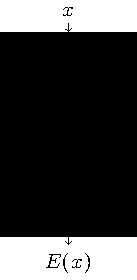
\includegraphics[width=3.5cm]{figures/blackbox.pdf}
    \end{textblock*}
}
\only<2>{
    \begin{textblock*}{4cm}(2cm,2cm)
    \begin{tabu} to 3.5cm { | X[c] | X[c]| }
 \hline
 $x$ & $E(x)$ \\ 
 \hline
 0 & 182 \\
 1 & 210 \\
 2 & 78 \\
 3 & 251 \\
 4 & 97 \\
%  5 & 83 \\
 \hline
 \multicolumn{2}{|c|}{\ldots} \\
 \hline
 252 & 112 \\
 253 & 19 \\
 254 & 224 \\
 255 & 74 \\
 \hline
\end{tabu}
    \end{textblock*}
}
\only<3->{
    \begin{textblock*}{4cm}(2cm,1.75cm)
        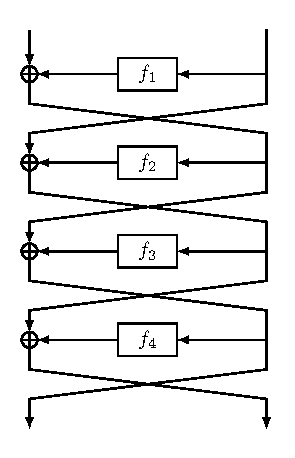
\includegraphics[height=5.75cm]{figures/feistel.pdf}
        \\
        \large \hspace*{0.3cm}
        Feistel Networks
    \end{textblock*}
    
}


\only<6>{
    \begin{textblock*}{4cm}(6.2cm,2cm)
    \begin{tabu} to 3.5cm { | X[c] | X[c]| }
 \hline
 $x$ & $E(x)$ \\ 
 \hline
 0 & 182 \\
 1 & 210 \\
 2 & 78 \\
 3 & 251 \\
 4 & 97 \\
%  5 & 83 \\
 \hline
 \multicolumn{2}{|c|}{\ldots} \\
 \hline
 252 & 112 \\
 253 & 19 \\
 254 & 224 \\
 255 & 74 \\
 \hline
\end{tabu}
    \end{textblock*}
}
\only<7->{
    \begin{textblock*}{4cm}(6cm,1.75cm)
    \begin{center}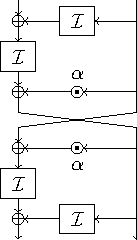
\includegraphics[height=5cm]{figures/apn.pdf}\end{center}
        \large
        \hspace*{1.1cm} 6-bit APN \\
        \hspace*{0.9cm} Permutation
    \end{textblock*}
}
\only<8->{
    \begin{textblock*}{6cm}(5.55cm,1.6cm)
        \begin{tikzpicture}
        \node[opacity=0.2] {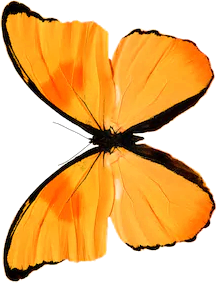
\includegraphics[height=6cm]{figures/butterfly.png}};
        \end{tikzpicture}
    \end{textblock*}
}

\only<4>{
    \begin{textblock*}{4cm}(10cm,2cm)
    \begin{tabu} to 3.5cm { | X[c] | X[c]| }
 \hline
 $x$ & $E(x)$ \\ 
 \hline
 0 & 182 \\
 1 & 210 \\
 2 & 78 \\
 3 & 251 \\
 4 & 97 \\
%  5 & 83 \\
 \hline
 \multicolumn{2}{|c|}{\ldots} \\
 \hline
 252 & 112 \\
 253 & 19 \\
 254 & 224 \\
 255 & 74 \\
 \hline
\end{tabu}
    \end{textblock*}
}
\only<5->{
    \begin{textblock*}{4cm}(10cm,1.75cm)
    \begin{center}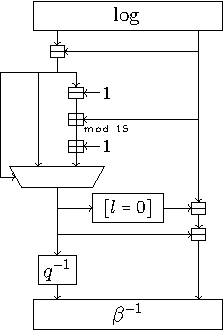
\includegraphics[height=5cm]{figures/kuzlog.pdf}\end{center}
        \large \hspace*{0.9cm}
        GOST S-Box
    \end{textblock*}
}

\end{frame}

\begin{frame}
    \CurTitle{}
    
    \nociteparti{mybibFeistel}
    \nociteparti{mybibAPN}
    \nociteparti{mybibKuz1}
    \nociteparti{mybibKuz2}
    \bibliographystyleparti{unsrt}
    \bibliographyparti{mybiblio.bib}
\end{frame}
\subsection{Nonlinear Invariant Cryptanalysis}

\renewcommand{\TITLE}{\it Nonlinear Invariant Cryptanalysis}

\begin{frame}[t]
\vspace{1.25cm}
\CurTitle{}

\Center{
    \textcolor{blue}{Properties} of messages that are \textcolor{green!70!black}{preserved} through encryption
}

\vspace{-0.5cm}

\only<2>{\Center{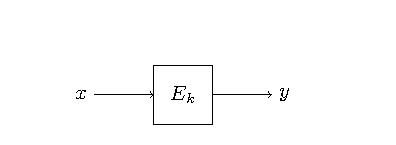
\includegraphics[height=3cm]{invariant1.pdf}}}
\only<3>{\Center{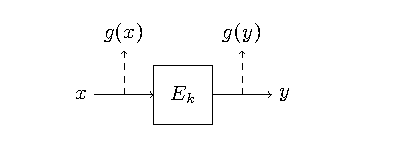
\includegraphics[height=3cm]{invariant2.pdf}}}
\only<4>{\Center{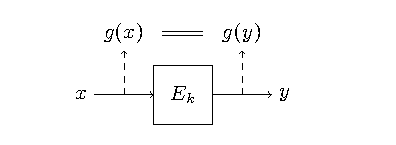
\includegraphics[height=3cm]{invariant3.pdf}}}
\only<5>{\Center{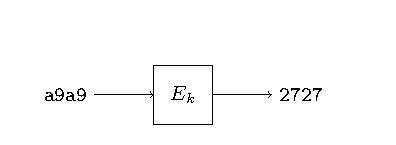
\includegraphics[height=3cm]{invariant4.pdf}}}
\only<6>{\Center{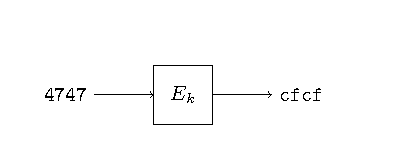
\includegraphics[height=3cm]{invariant5.pdf}}}
\end{frame}


\begin{frame}[t]
\CreditsTikz{}
\CurTitle{}

\Center{
\hspace*{1.75cm}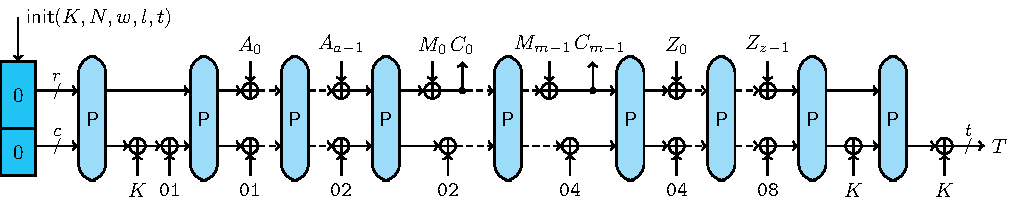
\includegraphics[width=0.85\linewidth]{norx_sponge_serial_v3.pdf}
}

\Block{4cm,4cm}{5cm}{
    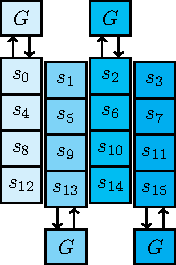
\includegraphics[width=2.5cm]{norx_G_col.pdf}
}
\Block{8cm,4cm}{5cm}{
    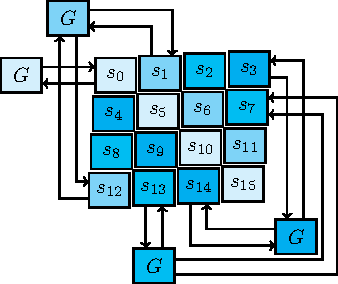
\includegraphics[width=4.5cm]{norx_G_diag.pdf}
}

\vspace{3.75cm}

\Center{
    \Large Analysis of the NORX Authenticated Encryption
}
\end{frame}


\begin{frame}[t]
\CurTitle{}

\vspace{1cm}

$$
\begin{bmatrix}
0 & 0 & 0 & 0 & 1 & 1 & 1 & 1 & 1 & 1 & 1 \\
0 & 1 & 1 & 1 & 0 & 0 & 0 & 1 & 1 & 1 & 1 \\
1 & 0 & 1 & 1 & 0 & 1 & 1 & 0 & 0 & 1 & 1 \\
1 & 1 & 0 & 1 & 1 & 0 & 1 & 0 & 1 & 0 & 1 \\
1 & 1 & 1 & 0 & 1 & 1 & 0 & 1 & 0 & 0 & 1 \\
\end{bmatrix}
$$

\vspace{0.5cm}

\Center{
    \Large Theoretical study of linear layers \\
    preserving degree-$d$ invariants
}
\end{frame}


\begin{frame}[t]
    \CurTitle{}
    
    \nocitepartii{mybibNORX}
    \nocitepartii{mybibNLI}
    \bibliographystylepartii{unsrt}
    \Block{3cm,2.5cm}{10cm}{
        \bibliographypartii{mybiblio.bib}
    }
\end{frame}

